
\documentclass[12pt,a4paper]{article}
\usepackage[latin1]{inputenc}
\usepackage{float}
\usepackage{amsmath}
\usepackage{amsfonts}
\usepackage{amssymb}
\usepackage{graphicx}
\usepackage[hidelinks]{hyperref}
\author{Giancarlo Danese - 945265\\
	Davide Savoldelli - 928676}
\date{A.Y. 2019/2020 - Prof. Di Nitto Elisabetta}


\title{
	\textbf{\Huge{SafeStreets}} \\
	\large Design Document
}

\begin{document}

	\begin{figure}
		\centering
		
\includegraphics[width=1.0\linewidth]{../assets/images/logo_poli.jpg}
	\end{figure}

	\maketitle
	\newpage
	\tableofcontents
	\newpage

\section{INTRODUCTION}
\subsection{Purpose}
This document represents the Design Document (DD) for SafeStreets software and contains a functional description of the system. Since we provide an overall guide of the systems' architecture, it's addressed to the software development team
\subsection{Scope}
SafeStreets will have an embedded algorithm which will analyze pictures of the vehicle plates sent by the user in order to recognize the vehicle. This information, together with the position of the vehicle and the type of violation that has been committed, will be stored in the software's database.
\newline
Authorities will have the chance to mine the information retrieved in the database by highlighting the streets/areas in which most of the violations are committed, the type of vehicles which commit most of the violations and which type of violations occur the most, suggesting possible interventions that could be taken.	
\subsection{Definitions, Acronyms, Abbreviations}
			\begin{itemize}
				\item \texttt{User Device}: any compatible device with the SafeStreets application, like a smartphone or a computer
				\item \texttt{Personal Information}: information provided by the user during the registration process. It includes name, surname, birth date, address, e-mail address, mobile number.
				\item \texttt{Violation Report}: the act in which users can denounce violations on the streets, by providing the system its position, a photo and by selecting a violation from a precompiled menu
				\item \texttt{Mobile App}: an application that can be run by mobile devices, both smartphones and smartwatches.
				\item \texttt{Violations Map}: a map, accessible only by authorities, which contains notifications and alerts about all the unsafe areas where several violations are committed
			\end{itemize}
		\subsubsection{Acronyms}
			\begin{itemize}
				\item RASD: Requirements Analysis and Specification Document.
				\item DD: Design Document
				\item API: Application Programming Interface.
				\item GPS: Global Positioning System.
				\item PRA: Pubblico Registro Automobilistico
				\item AUC: Authority Unique Code
				\item DBP: Device-bound PIN
			\end{itemize}
\subsection{Revision History}
\subsection{Reference Documents}
\subsection{Document Structure}
\begin{itemize}
\item \textbf{1 Introduction} 
This section introduces the Design Document. It explains the Purpose, the Scope and the framework of the document.
\item \textbf{2 Architectural Design}
This section is focused on the main components used for this system and the relationship between them, providing information about their deployment and how they operate. It also focuses on the architectural
styles and the design patterns adopted for designing the system.
\item \textbf{3 User Interface Design}
This section provides an overview on how the User Interface will look like. In our case this section won't be detailed since all the product
functions have been already represented in the RASD.
\item \textbf{4 Requirements Traceability}
This section explains how the requirements defined in the RASD map to the design elements defined in this document.
\item \textbf{5 Implementation, Integration and Test Plan}
In this section we identify the order in which we plan to implement the subcomponents of the system and the order in which we plan to
integrate and test them.
\end{itemize}
\newpage
\section{ARCHITECTURAL DESIGN}
\subsection{High-level components and their interaction}
\begin{figure}
		\centering
		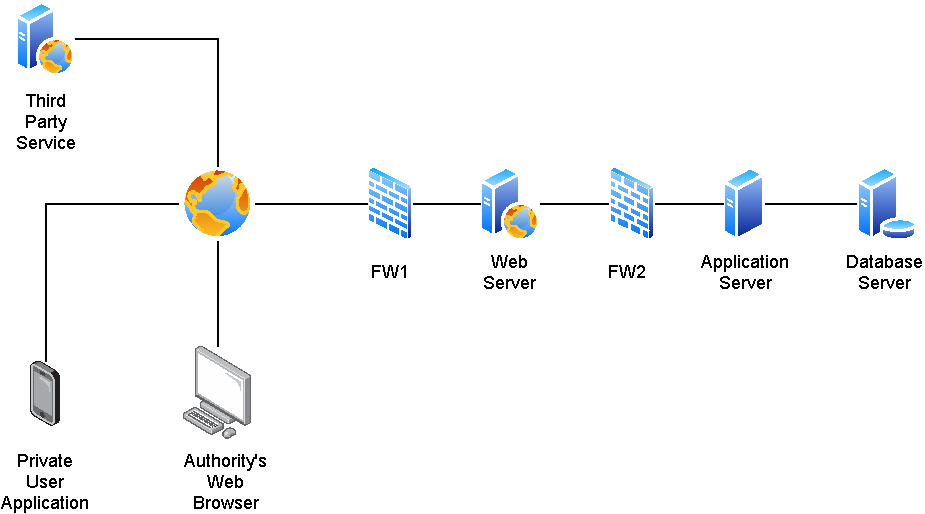
\includegraphics[width=1.0\linewidth]{../assets/sequence_diagrams/exports/architecture.pdf}
	\end{figure}
Our system can be summarized into 3 logical layers:
\begin{itemize}
\item \textbf{Presentation Layer}\\\\
This layer is divided into the Client tier (Mobile App for users) and the Web tier (Web App for authorities). From here, user, authorities and third parties, such as the municipality, can access the system's functionalities and the users' data through the Web Server, protected by a DeMilitarized Zone (DMZ)
\item \textbf{Application Layer}\\\\
In this layer the application server acts as a set of components accessible to the software developer through a standard API defined for the platform itself. We decided to separate the Application Server from the Web Server mainly for security reasons, and secondly because our application servers target much more than just Web page generation: they implement services like clustering, fail-over, and load-balancing.
\item \textbf{Data Layer}\\\\
Finally, here we have the Database Server and the Database itself, where all the data about the users, the authorities and the violations reported are stored and managed\\
\end{itemize}
A third-party ERP solution is how the System Administration is implemented, therefore we cannot provide information about its implementation
\subsection{Component view}
\subsubsection{High Level Component Diagram}
The following diagrams represents the systems' components and its interfaces throughout which they interact in order to execute their functionalities. We'll divide this view into two sides, the Client side and the Server side:
\begin{itemize}
\item The Client side is composed of two different components, the \texttt{Web Application}, intended for authorities only, and the \texttt{Mobile Application}, intended for the users. The former refers to the \texttt{AuthoritiesWebServices} service, the latter to the \texttt{UserMobileServices} service
\item The Server side is consequently also composed of two different components, the \texttt{Authorities Web Services} which will enable authorities to check the map, solve violations, etc., and the \texttt{User Mobile Services} which gives users the chance to report street/parking violations with pictures, check/modify their personal data and review their report history
\end{itemize}

\subsubsection{User Mobile Services Projection}
The User Mobile Services Projection is subdivided into 3 modules: the \texttt{User Access Module}, the \texttt{Violation Reporting Module},  and the \texttt{Reports History Module}
\subsubsection*{Module Functionalities}
\begin{itemize}
\item \textbf{User Access Module}: this module manages the registration and login processes of the user. It will allow them to insert their personal data and register to the system, and, subsequently, login with the same credentials.
\item \textbf{Violation Reporting Module}: this module is very important as it enables the user to report street/parking violations by taking pictures of the vehicle involved and uploading them to the system
\item \textbf{Reports History Module}: this module manages the users' report history, and, when requested, queries the data from the database and shows it to the user
\end{itemize}

\subsubsection{Authority Web Services Projection}
The Authority Web Services Projection is subdivided into 3 modules: the \texttt{Authority Access Module}, the \texttt{Violation Solving Module} and the \texttt{Suggestion Posting Module}
\begin{itemize}
\item \textbf{Authority Access Module}: this module manages the registration and login of the authority. It will allow them to insert their personal data and to receive their AUC and DBP in order to successfully register to the system.
\item \textbf{Violation Solving Module}: this module lets the authority interact with the list of violations, checking their validity and solving them. 
\item \textbf{Suggestion Posting Module}: this module manages the suggestions on possible interventions to take in order to prevent violations from being committed in that precise area.
\end{itemize}


\subsection{Deployment view}
In order to deploy the system, we decided to implement a 4-tier architecture:
\begin{itemize}
\item \textbf{Tier 1}
The first tier will be composed by the Client (we opted for a Thin Client) that includes a Mobile Application (for users) and a Web Application (for authorities).
\item \textbf{Tier 2}
This tier corresponds to the Web Server, whose main focus is to store, process static content and deliver web pages to the Clients. Infact, we opted for Apache Tomcat thanks to its high-availability, clustering feature for load balancing and its optimal java-focused environment
\item \textbf{Tier 3}
This tier corresponds to the Application Server, that both facilitates the creation of web applications and provides a server environment where to run these applications. We opted for Apache Geronimo, since one of its components is Tomcat, and because of its compatibility with Java EE 6 specifications.
\item \textbf{Tier 4}
The final tier corresponds to the Database Server, where the DBMS is running. We opted for MySQL, since it is one of the most secure and reliable database management system used in popular web applications, while at the same time guarantees scalability and high performance.
\end{itemize}
\subsection{Runtime view: You can use sequence diagrams to describe the way components interact to accomplish specific tasks typically related to your use cases}
\subsection{Component interfaces}
\subsection{Selected architectural styles and patterns}
\subsubsection{Design Patterns}
Here are the design patterns we used to make our architecture more flexible:
\begin{itemize}
\item \textbf{Model View Controller}
Nowadays, most Mobile and Web Applications rely on this pattern. These type of applications infact retrieve data from the Database and updates the Users' Interface consequently and according to the provided input, while the Controller checks the validity of the requested operations. Therefore the main scope of this pattern is to separate the Data (Model), the Users' Interface (View) and the user's input validator (Controller)
\item  \textbf{Observer and Observable}
\end{itemize}
\subsection{Other design decisions}
\section{USER INTERFACE DESIGN}
As already mentioned in the \texttt{Requirements Analysis and Specification Document} (RASD), our idea is to provide users with a Mobile App (for smartphones and tablets) and authorities with a Web App (for computers).\\ The applications will be different both in functionalities and in style, and we decided to separate the two and therefore make them exclusive, because of the different use and different authentication method they have.\\ For a closer look at what the two interfaces look like, we invite you to check our RASD where several mock-ups have been presented
\section{REQUIREMENTS TRACEABILITY: Explain how the requirements you have defined in the RASD map to the design elements that you have defined in this document.}
\section{IMPLEMENTATION, INTEGRATION AND TEST PLAN: Identify here the order in which you plan to implement the subcomponents of your system and the order in which you plan to integrate
such subcomponents and test the integration.}
\section{EFFORT SPENT}
\section{REFERENCES}



\end{document}